\chapter{はじめに}
\label{chapter: introduction}
所与の領域を一人または複数の巡査が動き回り,
その領域内の指定された場所を十分な頻度で訪れることを
警邏(patrolling)という\cite{
  Dumitrescu:2014:CGC:2636805.2636822,
  chen2013fence,
  coene2011charlemagne,
  czyzowicz2011boundary}.
\ncomment{[文献追加]}

本稿では,与えられた距離空間$U$内を速さ$1$以下の巡査$m$人が動きまわることにより,
集合$V \subseteq U$に属する多くの点に十分な頻度で訪れるという目標を考える.
すなわち次のような問題である.

巡査$i \in \{1, \ldots, m\}$の$U$上の運行$a _i \colon \Rset \to U$とは,
各時刻$t \in \Rset$における位置$a _i (t) \in U$を定めるものであって,
任意の時刻$s$,$t \in \Rset$に対し$a _i (s)$と$a _i (t)$の距離が$\abs{s - t}$を超えないものをいう.
巡査$m$人による$U$上の運行とは,
全巡査の運行を定めた組$A = (a _1, \dots, a _m)$をいう.
$U$の有限な部分集合$V$があり,$V$の各点には利得および{\maxIdletime}と呼ばれる正整数が定まっている.
点$v \in V$の{\maxIdletime}が$q$であるとき,
巡査達が運行$A = (a _1, \dots, a _m)$で点$v$を警備するとは,
長さ$q$のどの時間にも
いずれかの巡査が$v$を少なくとも一度は訪れる
(任意の時刻$t \in \Rset$に対して
巡査$i$と時刻$\tau \in [t, t + q)$が存在し$a _i (\tau) = v$)
ことをいう.
巡査達が運行$A$により点集合$W \subseteq V$を警邏するとは,
各点$v \in W$に対し巡査達が運行$A$で$v$を警備することをいう.
そのような運行が存在するとき$W$は$m$人により警邏可能であるという.

\begin{patrollingProblem}
  巡査の人数$m \in \Nset$と距離空間$U$内の点集合$V$および
  $V$の各点の利得と{\maxIdletime}が与えられる.
  $m$人の巡査により警邏可能な$V$の部分集合のうち
  利得の和が最大となるものを求めよ.
\end{patrollingProblem}

距離空間$U$といっても,$V$の点同士の測地距離のみが重要である.
そこで
$V = \{ v_1, \ldots, v_n \}$を点集合,
$q_1, \ldots, q_n$を$V$の各点の{\maxIdletime},
$p_1, \ldots, p_n$を$V$の各点の利得,
$d : V \times V \to \Rset$を$V$の2点間の距離として,
$(\{ (v_i, q_i, p_i) \mid i \in \{ 1, \ldots, n \} \}, d )$を\defword{地図}と呼び,
{\patProb}の入力は地図であるとする.

この問題は,巡査が一人かつ
全点の利得と{\maxIdletime}が等しい場合に限っても,
ハミルトン路問題からの帰着により
NP困難である\cite[Theorem~8]{coene2011charlemagne}.
そこでグラフの形状を限ったときにどのようになるかを調べる.

一つの点を複数の巡査の訪問により警備し得ることに注意されたい.
例えば図\ref{figure: cooperative}左はそのような運行の例である.
\begin{figure}
  \centering
  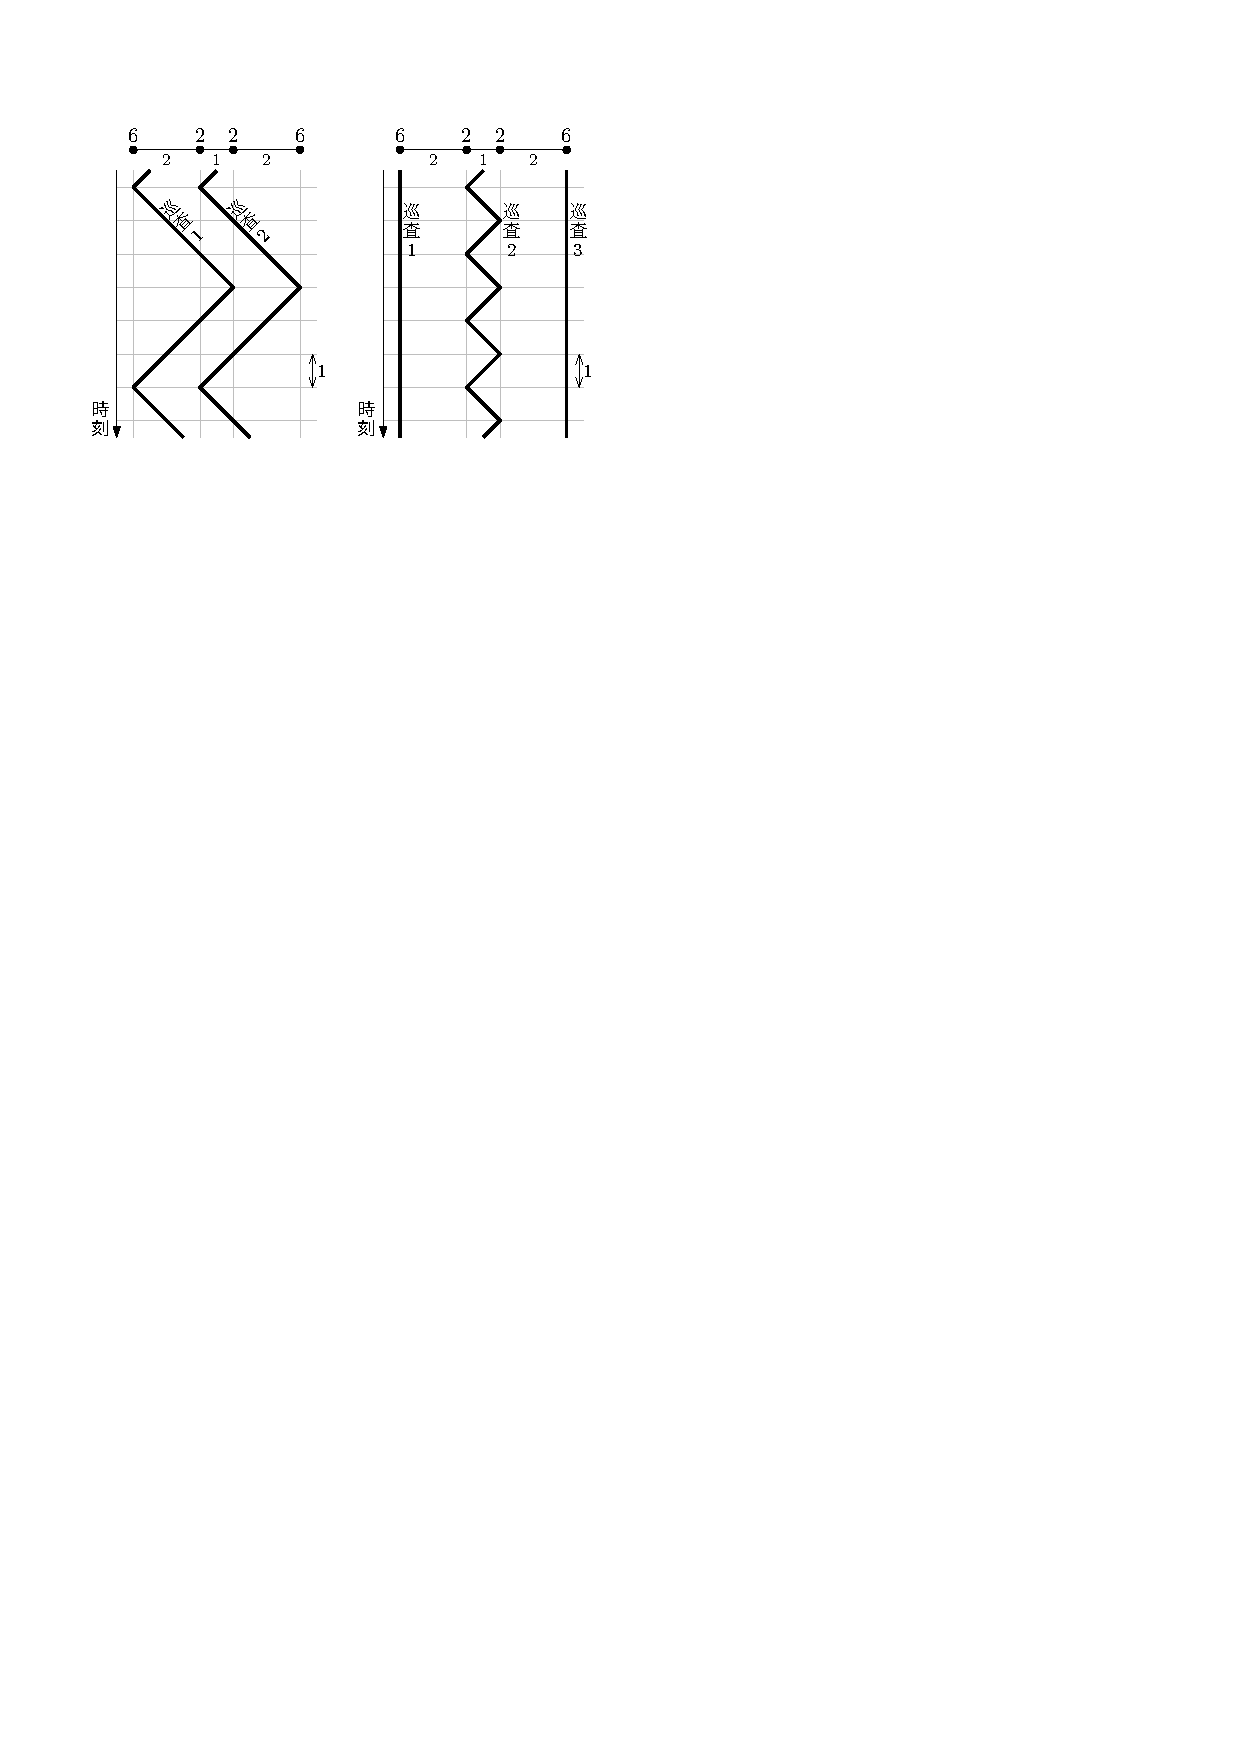
\includegraphics[scale=1.0]{\figdir/cooperative.pdf}
  \caption{図の上部に描かれている四点からなる{\graphLine}のグラフの全点を警邏する二つの運行.
    点と辺に書かれた数は,それぞれ{\maxIdletime}と距離である.
    左図の運行では二人の巡査が協力して中央の二点を間隔$2$で警備している.
    これを禁じ,各点がいずれかの巡査により単独警備されることを求める場合は,
    右図のように三人の巡査を要する.}
  \label{figure: cooperative}
\end{figure}
Coeneら\cite{coene2011charlemagne}は似た問題を扱っているが,
このような協力を許さず,
図\ref{figure: cooperative}右のように
各点を専ら一人の巡査が「担当」することを要求している.
つまり,各点$v \in W$が単独警備される(すなわち
或る一人の巡査がおり,
その巡査のみの運行が$v$を警備する)ことを要求しているのである.
対比のため本稿ではこの問題を{\independentPatProb}と呼ぶことにする
(\cite{coene2011charlemagne}ではMPLPPと称している).
Coeneら\cite{coene2011charlemagne}の諸結果においては,
この単独警備という限定が,
多項式時間算法の設計にも困難性の証明にも重要な役割を果している.
この限定を外したときの様子を調べるのが本稿の目的である.

本稿では地図の形状(即ち距離関数$d$の制約)として
線分,星と,すべての枝の長さが等しい完全グラフの3種類を扱うこととし
(図\ref{figure: graph_classes}),
以降はそれぞれを{\graphLine},{\graphStar},{\graphUnit}と呼ぶ.
\begin{figure}
  \centering
  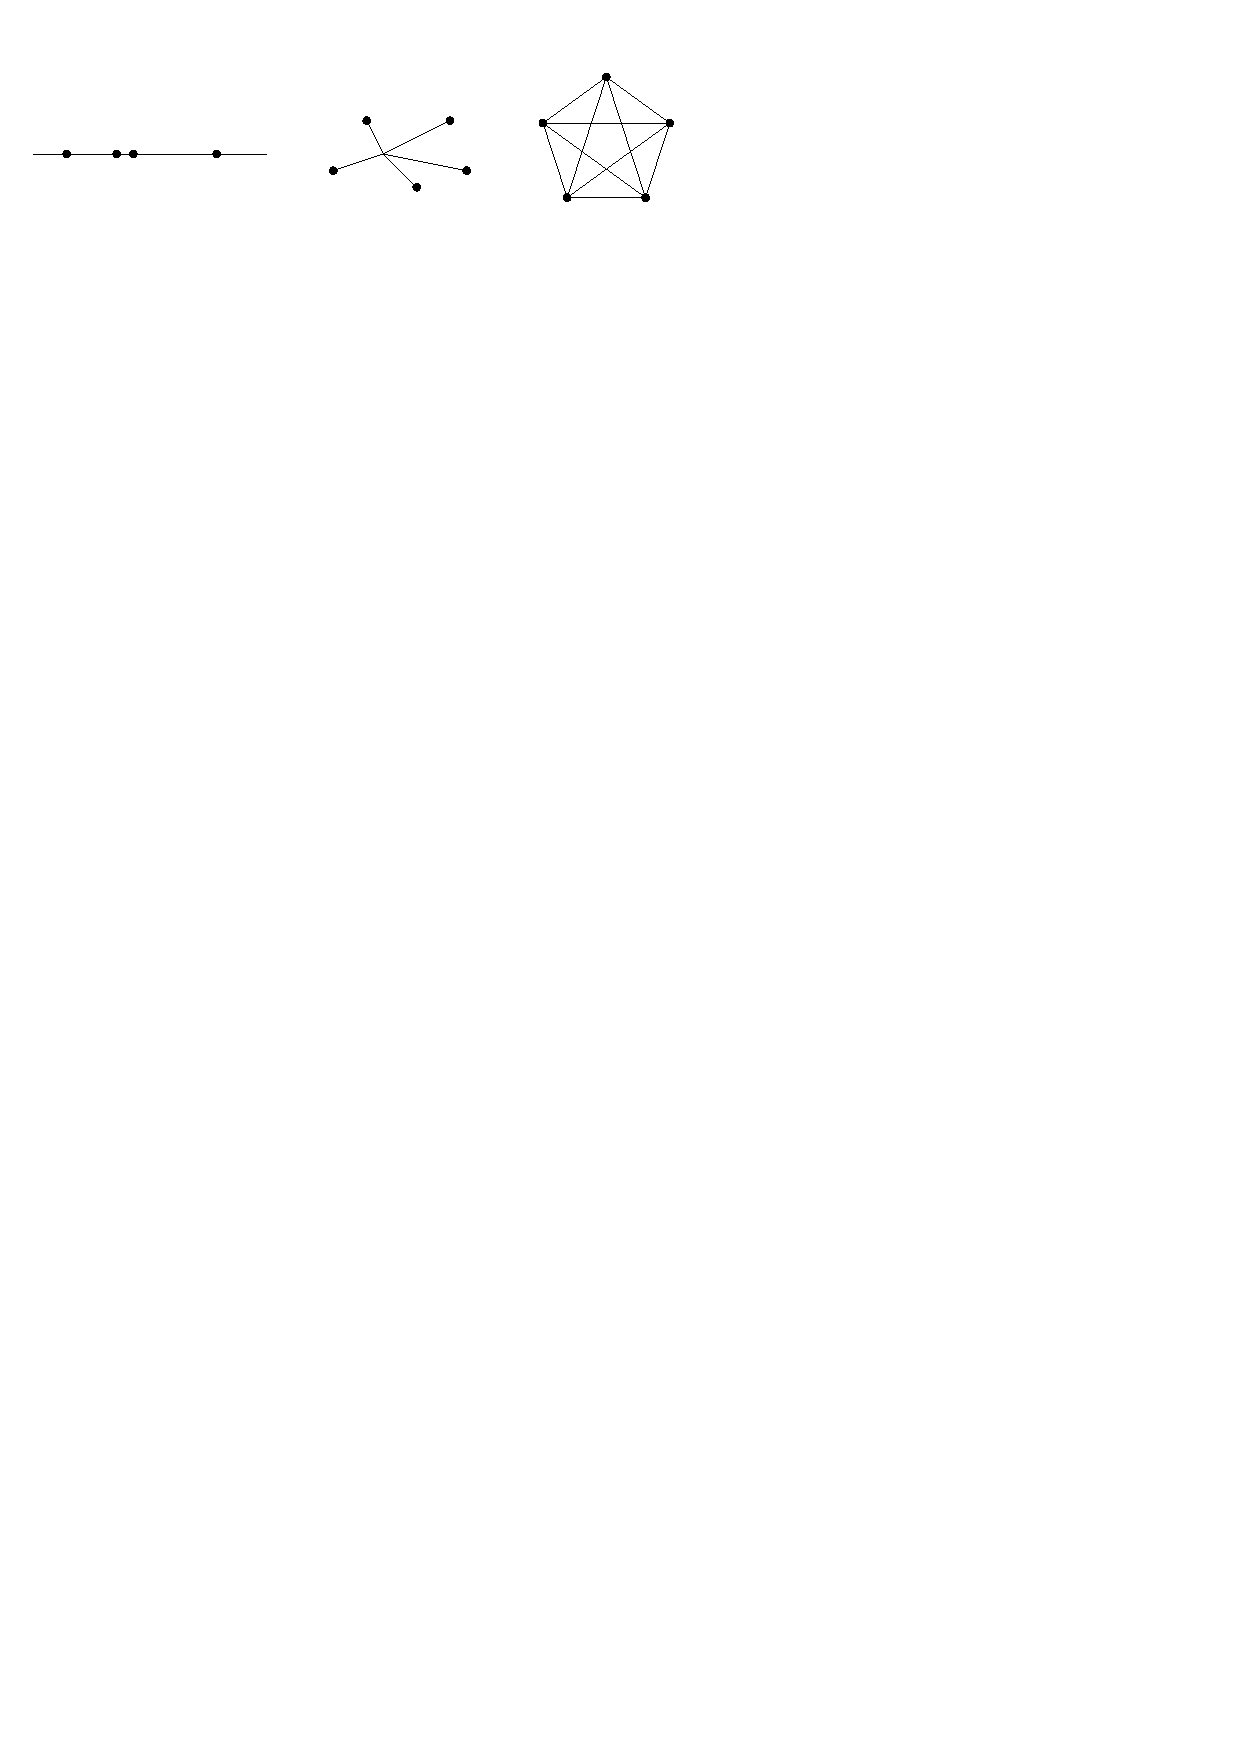
\includegraphics[scale=1.0]{\figdir/graph_classes.pdf}
  \caption{本論文では
    {\graphLine}(左),{\graphStar}(中),{\graphUnit}(右,但し各辺の長さが等しい)を扱う.
    {\graphStar}は葉のみを警備の対象とする(中央の点は移動の途中で使うのみであり,{\maxIdletime}は定められていない).}
  \label{figure: graph_classes}
\end{figure}
{\graphStar}では葉のみに{\maxIdletime}が定められている(中心は警備の対象としない).
{\graphUnit}のグラフはその辺の長さを$d$とすると,
同じ点数で辺の長さがすべて$d/2$である{\graphStar}のグラフの場合に帰着できることから,
{\graphUnit}は{\graphStar}の特殊な場合である.


{\patProb}についての我々の結果を
Coeneらの{\independentPatProb}についての結果との比較も含めて
グラフの形ごとにまとめると次のようになる.
それぞれ\ref{chapter: line},\ref{chapter: star},\ref{chapter: unit}節で述べる.
\begin{itemize}
\item 
  グラフが{\graphLine}の場合は,
  {\independentPatProb}は動的計画法により多項式時間で解けることが
  示されていた\cite[Theorem~11]{coene2011charlemagne}が,
  その正しさは単独警備という設定に強く依存している.
  本稿では{\patProb}について,
  全点の{\maxIdletime}が等しい場合には多項式時間で解けることを示す
  (定理\ref{theo:LineUnaryIdletime}).
\item
  グラフが{\graphStar}の場合は,
  全点の利得と{\maxIdletime}が等しい場合に限っても,
  {\independentPatProb}はNP困難であることが示されていた\cite[Theorem~10]{coene2011charlemagne}.
  本稿では,この場合の{\patProb}は多項式時間で解けるという興味深い結果を得る
  (定理\ref{theo:StarUnaryProfitAndIdletime}).
  なお利得または{\maxIdletime}を一般にすると,
  巡査が一人であっても(したがって独立かどうかによらず)
  NP困難であることがわかっている\cite[Theorems 5 and 6]{coene2011charlemagne}.
\item 
  グラフが{\graphUnit}の場合は,
  本稿では全点の{\maxIdletime}が等しい場合は{\patProb}が多項式時間で解けることを示す
  (定理\ref{theo:UnitUnaryIdletime}).
  グラフが{\graphStar}の場合は全点の{\maxIdletime}が等しくても利得が一般だとNP困難になるので,
  これにより{\graphUnit}は{\graphStar}よりも簡単に解ける場合となっていることが分かる.
\end{itemize}



グラフが{\graphLine}や{\graphUnit}の場合には,
全点の{\maxIdletime}が等しい場合には多項式時間で解けるのに対し,
{\maxIdletime}が一般の場合には多項式時間アルゴリズムを見つけることができなかった.
グラフが{\graphStar}の場合は{\patProb}がNP困難になる\cite{coene2011charlemagne}
ので,グラフが{\graphLine}や{\graphUnit}の場合についても
NP困難になるのではないかと予想したが,これも示すことができなかった.
これらの未解決な場合については,
{\maxIdletime}の代わりに{\exactIdletime}を警備の条件とする次のような問題を考えた.

\begin{defi}
  運行$A = (a _1, \ldots, a _m)$が点$v \in U$を
  {\exactIdletime}$(q, r) \in \Nset \times \Nset$で警備するとは,
  任意の時刻$t := q k + r\ (k \in \Zset)$に対し
  巡査$i$が存在し$a _i (t) = v$であることをいう.
\end{defi}

\begin{timeSpecifiedPatrollingProblem}
  巡査の人数$m$と距離空間$U$内の点集合$V$および各点の利得,
  警備の条件として{\exactIdletime}が与えられる.
  $m$人の巡査により警邏可能な$V$の部分集合のうち
  利得の和が最大となるものを求めよ.
\end{timeSpecifiedPatrollingProblem}

\begin{timeSpecifiedPatrollingProblemDecision}
  巡査の人数$m$と距離空間$U$内の点集合$V$および
  警備の条件として各点の{\exactIdletime}が与えられる.
  $m$人の巡査により$V$を警邏可能か判定せよ.
\end{timeSpecifiedPatrollingProblemDecision}


{\graphLine}については{\timeSpecifiedPatProbDecision}を解く貪欲アルゴリズムを示す(定理\ref{theo:LineTimeSpecifiedGreedy}).
{\graphUnit}については{\timeSpecifiedPatProb}がNP困難であることを示す(定理\ref{theo:UnitExacIdletimeNPhard}).
